\chapter{Restrições do Projecto}
\minitoc
\section{Restrições impostas}
\subsection{Restrições de Solução}
    A \textit{appliance} que irá ser desenvolvida está restrita a duas topologias de instalação distintas, as quais dependem da infraestrutura de rede onde o produto será montado. A escalabilidade e a performance da rede são os principais factores que levaram à concepção destas duas soluções. \\

    A topologia apresentada na Figura ~\ref{img:topo1} é uma solução mais simples, mais genérica, podendo ser considerada uma solução \textit{plug-and-play}, uma vez que não são necessárias configurações de rede onde o \textit{Delusion} será montado. Esta é uma solução que tem como objectivo servir um número limitado de utilizadores, dado que a sua performance decai consideravelmente com o aumentar do trâfego de rede. \\

\begin{figure}
	\centering	
	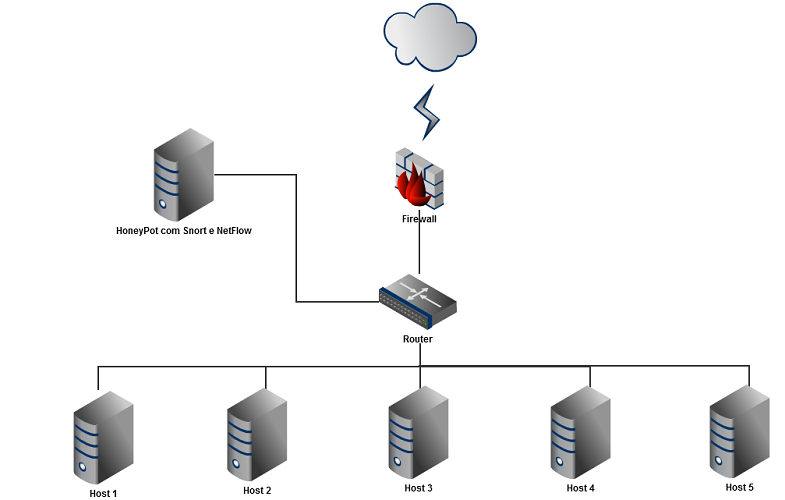
\includegraphics[scale=0.6]{images/topologia1.png}
	\caption{Topologia de Rede Plug-and-Play}
    \label{img:topo1}
\end{figure}

    A segunda topologia, ilustrada na Figura ~\ref{img:topo2}, é uma solução mais escalavel, não tendo um número máximo de utilizadores que consegue servir. Portanto, esta solução tem como objectivo servir uma infraestrutura de rede com dimensões maiores do que a primeira topologia. Como se pode observar na Figura ~\ref{img:topo2}, esta solução divide a infraestrutura de rede em várias subredes, sendo instalado em cada uma um \textit{sniffer} que irá detectar as intrusões sucedidas nesse segmento de rede.

\begin{figure}
	\centering	
	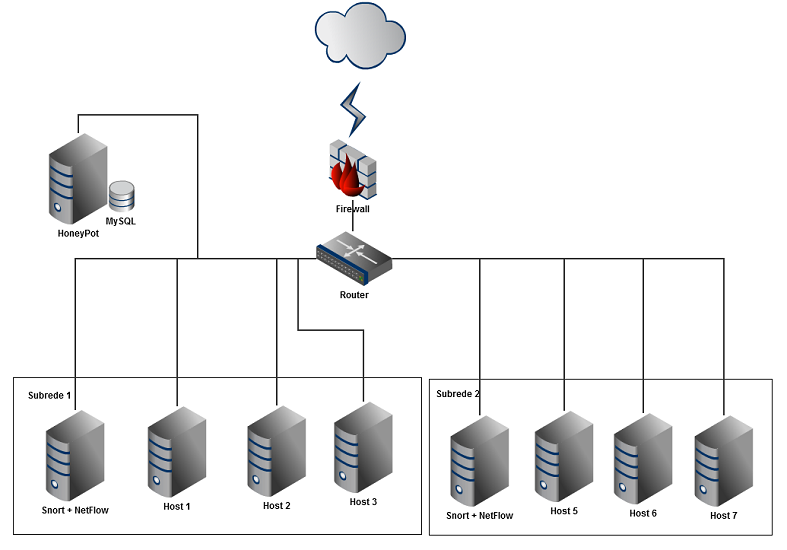
\includegraphics[scale=0.6]{images/topologia3.png}
	\caption{Topologia de Rede Escalavel}
    \label{img:topo2}
\end{figure}


\subsection{Ambiente de Instalação do Sistema}

    O \textit{Delusion} é um produto que será instalado consoante as necessidades de cada cliente, assim como já foi referido nas restrições de solução.

\subsection{Software Off-the-Shelf}
\begin{description}
    \item [Visual Paradigm for UML 7.1 Community Edition] usado para modelar o sistema de negócio e o sistema informático
    \item [Snort] Sistema de detecçã de intrusões
    \item [Netflow] Colector de informações de trâfego
    \item [IpTables] Ferramenta para configurar as tabelas da firewall do kernel
    \item [Nmap] Scanner de segurança
    \item [Ruby on Rails] Framework de desenvolvimento web da linguagem \textit{Ruby}
    \item [Tshark] Visualizador da linha de comandos do trâfego capturado pelo \textit{Wireshark}
    \item [Wireshark] Analisador de pacotes de rede
\end{description}

\subsection{Ambiente de Trabalho}

    O \textit{Delusion} terá como interface um ambiente \textit{web} que permita aos administradores de sistema configurar serviços e observar os vários eventos que sucederam na rede. O acesso a esta interface \textit{web} terá que ser estabelecido através de uma ligação segura, garantindo a confidencialidade, integridade e autenticidade dos dados que serão transmitidos.\\

    Devido as características únicas de configuração e visualização que o \textit{Delusion} proporciona, o acesso aos seus serviços será restrito à \textit{intranet}, não sendo permitidos acessos do exterior (\textit{internet}) por questões de protecção e segurança.

\subsection{Restrições de Calendário}
\begin{description}
    \item 12 de Novembro de 2011 - Visão do Produto: 
        \begin{itemize}
            \item Análise de mercado
            \item Modelo de negócio, proposta de valor e avaliação da oportunidade
            \item Documento de Requisitos
        \end{itemize}
    \item 14 de Janeiro de 2012 - Documentação Técnica e de Instalação: 
        \begin{itemize}
            \item Produto de software
            \item Manuais de utilização
        \end{itemize}
    \item 11 de Fevereiro de 2012 : Visão Final do Produto:
        \begin{itemize}
            \item Documento de Requisitos
            \item Plano do projecto
            \item Documento do estado do projecto
            \item Documentação técnica e de instalação
            \item Produto de software
            \item Manuais de utilização
        \end{itemize}
    \item 18 de Fevereiro de 2012 : Apresentação Final: 
        \begin{itemize}
            \item Apresentação final
            \item Exposição dos trabalhos
        \end{itemize}
\end{description}

\section{Nomenclatura e Definições}
\subsection{Termos Usados no Projecto}

    Ver Anexo ~\ref{appendix:1}.
